%%%%%%%%%%%%%%%%%%%%%%%%%%%%%%%%%%%%%%%%%%%%%%%%%%%%%%%%%%%%%%%%%
%2345678901234567890123456789012345678901234567890123456789012345
%        1         2         3         4         5         6     
\chapter{Mobile robot control framework}
\label{cha:framework}
A mobile robot is a complex system with several functional block. From control perspect of view, the system can be roughly divided into 2 parts, global planner and local planner.
Within this study we focus on the local planner which takes the task space velocity and acceleration command $\dot{\xi},\ddot{\xi}$ as input and calculate the corresponding optimal joint response, coordinate the steering and driving of four wheels, Which include 4 steering motors and 4 driving motors. The local planner communicate with these motors with CAN bus at 1 KHz, and take the task space command from global planner with ROS network at the same time.
The other part of the system is the global planner, which is responsible to sense the environment and make decision to plan the trajectory. It is out of scope of this paper, we just simplify it as a node which output task space command at 20Hz.


%%%%%%%%%%%%%%%%%%%%%%%%%%%%%%%%%%%%%%%%%%%%%%%%%%%%%%%%%%%%%%%%%%%%%%%%%%%%%%%%%%%%%%%%%%%%%%%%%%%%%%%%%%%%%%%%%%%%%%%%%%%%%%%%%%%%%%%%%%%%%%%%%%%%%%%%%%%%%%%%%%%%%%%%%%%%%%%%%%%%%%%%%%%%%%%%

\tikzstyle{myarrow}=[->, thick]
\tikzstyle{line}=[-, thick]
\begin{figure}[t]\label{fig:hardwareStructure}
	\begin{center}
		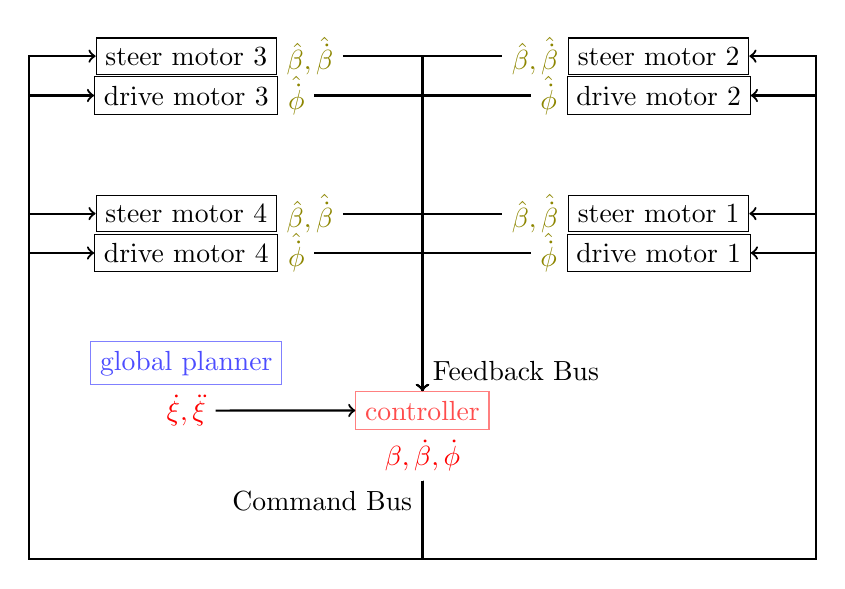
\begin{tikzpicture}
		    \node (global planner) at (-3, 0.6) [rectangle, draw=blue!50, text=blue!70, label={[name=task command, red]-90:$\dot{\xi},\ddot{\xi}$}] {global planner};
		    \node (controller) at (0, 0) [rectangle, draw=red!50, text=red!70, label={[name=command, red]-90:$\beta,\dot{\beta},\dot{\phi}$}] {controller};
		    
			\node (steer1) at (3, 2.5) [rectangle, draw=black, label={[name=steer1Feedback, olive]180:$\hat{\beta},\hat{\dot{\beta}}$}] {steer motor 1};
			\node (drive1) at (3, 2) [rectangle, draw=black, label={[name=drive1Feedback, olive]180:$\hat{\dot{\phi}}$}] {drive motor 1};
			\draw[myarrow] (steer1Feedback) -| (controller.north);
			\draw[line] (drive1Feedback) -| (controller.north);

            \node (steer2) at (3, 4.5) [rectangle, draw=black, label={[name=steer2Feedback, olive]180:$\hat{\beta},\hat{\dot{\beta}}$}] {steer motor 2};
			\node (drive2) at (3, 4) [rectangle, draw=black, label={[name=drive2Feedback, olive]180:$\hat{\dot{\phi}}$}] {drive motor 2};
			\draw[myarrow] (steer2Feedback) -| (controller.north);
			\draw[line] (drive2Feedback) -| (controller.north);
			
			\node (steer3) at (-3, 4.5) [rectangle, draw=black, label={[name=steer3Feedback, olive]0:$\hat{\beta},\hat{\dot{\beta}}$}] {steer motor 3};
			\node (drive3) at (-3, 4) [rectangle, draw=black, label={[name=drive3Feedback, olive]0:$\hat{\dot{\phi}}$}] {drive motor 3};
			\draw[myarrow] (steer3Feedback) -| (controller.north);
			\draw[line] (drive3Feedback) -| (controller.north);
			
			\node (steer4) at (-3, 2.5) [rectangle, draw=black, label={[name=steer4Feedback, olive]0:$\hat{\beta},\hat{\dot{\beta}}$}] {steer motor 4};
			\node (drive4) at (-3, 2) [rectangle, draw=black, label={[name=drive4Feedback, olive]0:$\hat{\dot{\phi}}$}] {drive motor 4};
			\draw[myarrow] (steer4Feedback) -| (controller.north);
			\draw[line] (drive4Feedback) -| (controller.north) node[anchor=south west] {Feedback Bus};
			
			\draw[myarrow] (command.south) -- ++ (0,-1) -- ++(5,0)-- ++(0, 2) |- (steer1.east);
			\draw[myarrow] (command.south) -- ++ (0,-1) -- ++(5,0)-- ++(0, 2) |- (drive1.east);
			\draw[myarrow] (command.south) -- ++ (0,-1) -- ++(5,0)-- ++(0, 2) |- (steer2.east);
			\draw[myarrow] (command.south) -- ++ (0,-1) -- ++(5,0)-- ++(0, 2) |- (drive2.east);
			\draw[myarrow] (command.south) -- ++ (0,-1) -- ++(-5,0)-- ++(0, 2) |- (steer3.west);
			\draw[myarrow] (command.south) -- ++ (0,-1) -- ++(-5,0)-- ++(0, 2) |- (drive3.west);
			\draw[myarrow] (command.south) -- ++ (0,-1) -- ++(-5,0)-- ++(0, 2) |- (steer4.west);
			\draw[myarrow] (command.south) node[anchor=north east] {Command Bus} -- ++ (0,-1) -- ++(-5,0)-- ++(0, 2) |- (drive4.west);
			\draw[myarrow] (task command)--(controller.west);
		\end{tikzpicture}
	\end{center}
	\caption{System inter-connection}
\end{figure}


%%%%%%%%%%%%%%%%%%%%%%%%%%%%%%%%%%%%%%%%%%%%%%%%%%%%%%%%%%%%%%%%%%%%%%%%%%%%%%%%%%%%%%%%%%%%%%%%%%%%%%%%%%%%%%%%%%%%%%%%%%%%%%%%%%%%%%%%%%%%%%%%%%%%%%%%%%%%%%%%%%%%%%%%%%%%%%%%%%%%%%%%%%%%%%%%

\section{Low-level controller structure}
\label{sec:structure}
\tikzstyle{myarrow}=[->, thick]
\tikzstyle{line}=[-, thick]
\begin{figure}[t]\label{fig:controller}
	\begin{center}
		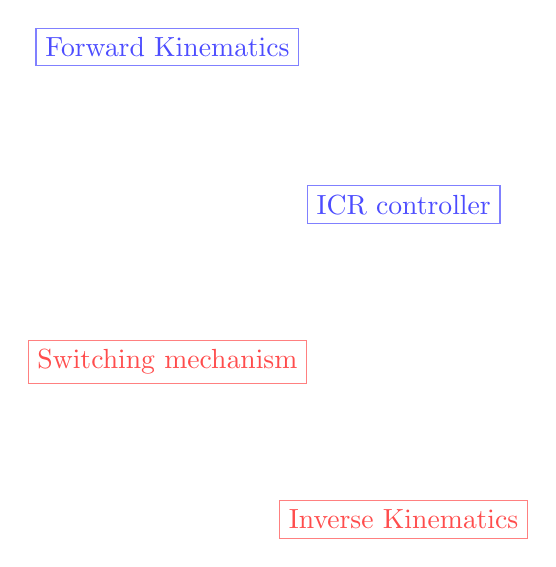
\begin{tikzpicture}
		    \node (FKAM) at (-2, 4) [rectangle, draw=blue!50, text=blue!70] {Forward Kinematics};
		    \node (switch) at (-2, 0) [rectangle, draw=red!50, text=red!70] {Switching mechanism};
		    \node (ICR) at (1, 2) [rectangle, draw=blue!50, text=blue!70] {ICR controller};
		    \node (IKAM) at (1, -2) [rectangle, draw=red!50, text=red!70] {Inverse Kinematics};
		    
		\end{tikzpicture}
	\end{center}
	\caption{Low-level controller structure}
\end{figure}
%%%%%%%%%%%%%%%%%%%%%%%%%%%%%%%%%%%%%%%%%%%%%%%%%%%%%%%%%%%%%%%%%%%%%%%%%%%%%%%%%%%%%%%%%%%%%%%%%%%%%%%%%%%%%%%%%%%%%%%%%%%%%%%%%%%%%%%%%%%%%%%%%%%%%%%%%%%%%%%%%%%%%%%%%%%
